\documentclass[a4paper]{article}

\def\npart {III}
\def\nterm {Lent}
\def\nyear {2017}
\def\nlecturer {A. G. Kovalev}
\def\ncourse {Riemannian Geometry}
\def\nlectures {TTS.12}

% Imports
\ifx \nextra \undefined
  \usepackage[pdftex,
    hidelinks,
    pdfauthor={Dexter Chua},
    pdfsubject={Cambridge Maths Notes: Part \npart\ - \ncourse},
    pdftitle={Part \npart\ - \ncourse},
  pdfkeywords={Cambridge Mathematics Maths Math \npart\ \nterm\ \nyear\ \ncourse}]{hyperref}
  \title{Part \npart\ - \ncourse}
\else
  \usepackage[pdftex,
    hidelinks,
    pdfauthor={Dexter Chua},
    pdfsubject={Cambridge Maths Notes: Part \npart\ - \ncourse\ (\nextra)},
    pdftitle={Part \npart\ - \ncourse\ (\nextra)},
  pdfkeywords={Cambridge Mathematics Maths Math \npart\ \nterm\ \nyear\ \ncourse\ \nextra}]{hyperref}

  \title{Part \npart\ - \ncourse \\ {\Large \nextra}}
\fi

\author{Lectured by \nlecturer \\\small Notes taken by Dexter Chua}
\date{\nterm\ \nyear}

\usepackage{alltt}
\usepackage{amsfonts}
\usepackage{amsmath}
\usepackage{amssymb}
\usepackage{amsthm}
\usepackage{booktabs}
\usepackage{caption}
\usepackage{enumitem}
\usepackage{fancyhdr}
\usepackage{graphicx}
\usepackage{mathtools}
\usepackage{microtype}
\usepackage{multirow}
\usepackage{pdflscape}
\usepackage{pgfplots}
\usepackage{siunitx}
\usepackage{tabularx}
\usepackage{tikz}
\usepackage{tkz-euclide}
\usepackage[normalem]{ulem}
\usepackage[all]{xy}

\pgfplotsset{compat=1.12}

\pagestyle{fancyplain}
\lhead{\emph{\nouppercase{\leftmark}}}
\ifx \nextra \undefined
  \rhead{
    \ifnum\thepage=1
    \else
      \npart\ \ncourse
    \fi}
\else
  \rhead{
    \ifnum\thepage=1
    \else
      \npart\ \ncourse\ (\nextra)
    \fi}
\fi
\usetikzlibrary{arrows}
\usetikzlibrary{decorations.markings}
\usetikzlibrary{decorations.pathmorphing}
\usetikzlibrary{positioning}
\usetikzlibrary{fadings}
\usetikzlibrary{intersections}
\usetikzlibrary{cd}

\newcommand*{\Cdot}{\raisebox{-0.25ex}{\scalebox{1.5}{$\cdot$}}}
\newcommand {\pd}[2][ ]{
  \ifx #1 { }
    \frac{\partial}{\partial #2}
  \else
    \frac{\partial^{#1}}{\partial #2^{#1}}
  \fi
}

% Theorems
\theoremstyle{definition}
\newtheorem*{aim}{Aim}
\newtheorem*{axiom}{Axiom}
\newtheorem*{claim}{Claim}
\newtheorem*{cor}{Corollary}
\newtheorem*{defi}{Definition}
\newtheorem*{eg}{Example}
\newtheorem*{fact}{Fact}
\newtheorem*{law}{Law}
\newtheorem*{lemma}{Lemma}
\newtheorem*{notation}{Notation}
\newtheorem*{prop}{Proposition}
\newtheorem*{thm}{Theorem}

\renewcommand{\labelitemi}{--}
\renewcommand{\labelitemii}{$\circ$}
\renewcommand{\labelenumi}{(\roman{*})}

\let\stdsection\section
\renewcommand\section{\newpage\stdsection}

% Strike through
\def\st{\bgroup \ULdepth=-.55ex \ULset}

% Maths symbols
\newcommand{\bra}{\langle}
\newcommand{\ket}{\rangle}

\newcommand{\N}{\mathbb{N}}
\newcommand{\Z}{\mathbb{Z}}
\newcommand{\Q}{\mathbb{Q}}
\renewcommand{\H}{\mathbb{H}}
\newcommand{\R}{\mathbb{R}}
\newcommand{\C}{\mathbb{C}}
\newcommand{\Prob}{\mathbb{P}}
\renewcommand{\P}{\mathbb{P}}
\newcommand{\E}{\mathbb{E}}
\newcommand{\F}{\mathbb{F}}
\newcommand{\cU}{\mathcal{U}}
\newcommand{\RP}{\mathbb{RP}}
\newcommand{\CP}{\mathbb{CP}}

\newcommand{\ph}{\,\cdot\,}

\DeclareMathOperator{\sech}{sech}
\DeclareMathOperator{\cosech}{cosech}
\DeclareMathOperator{\cosec}{cosec}

\DeclareMathOperator{\covol}{covol}
\DeclareMathOperator{\vol}{vol}

\let\Im\relax
\let\Re\relax
\DeclareMathOperator{\Im}{Im}
\DeclareMathOperator{\Re}{Re}
\DeclareMathOperator{\im}{im}
\DeclareMathOperator{\image}{image}
\DeclareMathOperator{\Ann}{Ann}

\DeclareMathOperator*{\res}{res}
\DeclareMathOperator{\Res}{Res}
\DeclareMathOperator{\Ind}{Ind}

\DeclareMathOperator{\tr}{tr}
\DeclareMathOperator{\diag}{diag}
\DeclareMathOperator{\rank}{rank}
\DeclareMathOperator{\card}{card}
\DeclareMathOperator{\spn}{span}
\DeclareMathOperator{\adj}{adj}

\DeclareMathOperator{\erf}{erf}
\DeclareMathOperator{\erfc}{erfc}

\DeclareMathOperator{\ord}{ord}
\DeclareMathOperator{\Sym}{Sym}

\DeclareMathOperator{\sgn}{sgn}
\DeclareMathOperator{\orb}{orb}
\DeclareMathOperator{\stab}{stab}
\DeclareMathOperator{\ccl}{ccl}

\DeclareMathOperator{\lcm}{lcm}
\DeclareMathOperator{\hcf}{hcf}

\DeclareMathOperator{\Int}{Int}
\DeclareMathOperator{\id}{id}

\DeclareMathOperator{\betaD}{beta}
\DeclareMathOperator{\gammaD}{gamma}
\DeclareMathOperator{\Poisson}{Poisson}
\DeclareMathOperator{\binomial}{binomial}
\DeclareMathOperator{\multinomial}{multinomial}
\DeclareMathOperator{\Bernoulli}{Bernoulli}
\DeclareMathOperator{\like}{like}

\DeclareMathOperator{\var}{var}
\DeclareMathOperator{\cov}{cov}
\DeclareMathOperator{\bias}{bias}
\DeclareMathOperator{\mse}{mse}
\DeclareMathOperator{\corr}{corr}

\DeclareMathOperator{\otp}{otp}
\DeclareMathOperator{\dom}{dom}

\DeclareMathOperator{\Root}{Root}
\DeclareMathOperator{\supp}{supp}
\DeclareMathOperator{\rel}{rel}
\DeclareMathOperator{\Hom}{Hom}
\DeclareMathOperator{\Aut}{Aut}
\DeclareMathOperator{\Gal}{Gal}
\DeclareMathOperator{\Mat}{Mat}
\DeclareMathOperator{\End}{End}
\DeclareMathOperator{\Char}{char}
\DeclareMathOperator{\ev}{ev}
\DeclareMathOperator{\St}{St}
\DeclareMathOperator{\Lk}{Lk}
\DeclareMathOperator{\disc}{disc}
\DeclareMathOperator{\Isom}{Isom}
\DeclareMathOperator{\length}{length}
\DeclareMathOperator{\energy}{energy}
\DeclareMathOperator{\area}{area}
\DeclareMathOperator{\Syl}{Syl}
\DeclareMathOperator{\cl}{cl}
\DeclareMathOperator{\fix}{fix}

\newcommand{\GL}{\mathrm{GL}}
\newcommand{\SL}{\mathrm{SL}}
\newcommand{\PGL}{\mathrm{PGL}}
\newcommand{\PSL}{\mathrm{PSL}}
\newcommand{\PSU}{\mathrm{PSU}}
\newcommand{\Or}{\mathrm{O}}
\newcommand{\SO}{\mathrm{SO}}
\newcommand{\U}{\mathrm{U}}
\newcommand{\SU}{\mathrm{SU}}

\renewcommand{\d}{\mathrm{d}}
\newcommand{\D}{\mathrm{D}}

\tikzset{->/.style = {decoration={markings,
                                  mark=at position 1 with {\arrow[scale=2]{latex'}}},
                      postaction={decorate}}}
\tikzset{<-/.style = {decoration={markings,
                                  mark=at position 0 with {\arrowreversed[scale=2]{latex'}}},
                      postaction={decorate}}}
\tikzset{<->/.style = {decoration={markings,
                                   mark=at position 0 with {\arrowreversed[scale=2]{latex'}},
                                   mark=at position 1 with {\arrow[scale=2]{latex'}}},
                       postaction={decorate}}}
\tikzset{->-/.style = {decoration={markings,
                                   mark=at position #1 with {\arrow[scale=2]{latex'}}},
                       postaction={decorate}}}
\tikzset{-<-/.style = {decoration={markings,
                                   mark=at position #1 with {\arrowreversed[scale=2]{latex'}}},
                       postaction={decorate}}}

\tikzset{circ/.style = {fill, circle, inner sep = 0, minimum size = 3}}
\tikzset{mstate/.style={circle, draw, blue, text=black, minimum width=0.7cm}}

\definecolor{mblue}{rgb}{0.2, 0.3, 0.8}
\definecolor{morange}{rgb}{1, 0.5, 0}
\definecolor{mgreen}{rgb}{0.1, 0.4, 0.2}
\definecolor{mred}{rgb}{0.5, 0, 0}

\def\drawcirculararc(#1,#2)(#3,#4)(#5,#6){%
    \pgfmathsetmacro\cA{(#1*#1+#2*#2-#3*#3-#4*#4)/2}%
    \pgfmathsetmacro\cB{(#1*#1+#2*#2-#5*#5-#6*#6)/2}%
    \pgfmathsetmacro\cy{(\cB*(#1-#3)-\cA*(#1-#5))/%
                        ((#2-#6)*(#1-#3)-(#2-#4)*(#1-#5))}%
    \pgfmathsetmacro\cx{(\cA-\cy*(#2-#4))/(#1-#3)}%
    \pgfmathsetmacro\cr{sqrt((#1-\cx)*(#1-\cx)+(#2-\cy)*(#2-\cy))}%
    \pgfmathsetmacro\cA{atan2(#2-\cy,#1-\cx)}%
    \pgfmathsetmacro\cB{atan2(#6-\cy,#5-\cx)}%
    \pgfmathparse{\cB<\cA}%
    \ifnum\pgfmathresult=1
        \pgfmathsetmacro\cB{\cB+360}%
    \fi
    \draw (#1,#2) arc (\cA:\cB:\cr);%
}
\newcommand\getCoord[3]{\newdimen{#1}\newdimen{#2}\pgfextractx{#1}{\pgfpointanchor{#3}{center}}\pgfextracty{#2}{\pgfpointanchor{#3}{center}}}

\def\Xint#1{\mathchoice
   {\XXint\displaystyle\textstyle{#1}}%
   {\XXint\textstyle\scriptstyle{#1}}%
   {\XXint\scriptstyle\scriptscriptstyle{#1}}%
   {\XXint\scriptscriptstyle\scriptscriptstyle{#1}}%
   \!\int}
\def\XXint#1#2#3{{\setbox0=\hbox{$#1{#2#3}{\int}$}
     \vcenter{\hbox{$#2#3$}}\kern-.5\wd0}}
\def\ddashint{\Xint=}
\def\dashint{\Xint-}


\begin{document}
\maketitle
{\small
\setlength{\parindent}{0em}
\setlength{\parskip}{1em}
This course is a possible natural sequel of the course Differential Geometry offered in Michaelmas Term. We shall explore various techniques and results revealing intricate and subtle relations between Riemannian metrics, curvature and topology. I hope to cover much of the following:

\emph{A closer look at geodesics and curvature.} Brief review from the Differential Geometry course. Geodesic coordinates and Gauss' lemma. Jacobi fields, completeness and the Hopf--Rinow theorem. Variations of energy, Bonnet--Myers diameter theorem and Synge's theorem.

\emph{Hodge theory and Riemannian holonomy.} The Hodge star and Laplace--Beltrami operator. The Hodge decomposition theorem (with the `geometry part' of the proof). Bochner--Weitzenock formulae. Holonomy groups. Interplays with curvature and de Rham cohomology.

\emph{Ricci curvature.} Fundamental groups and Ricci curvature. The Cheeger--Gromoll splitting theorem.

\subsubsection*{Pre-requisites}
Manifolds, differential forms, vector fields. Basic concepts of Riemannian geometry (curvature, geodesics etc.) and Lie groups. The course Differential Geometry offered in Michaelmas Term is the ideal pre-requisite.
}
\tableofcontents

\section{Basics of Riemannian manifolds}
This will be a very brief summary of some topics in the Michaelmas Differential Geometry course.

\begin{defi}[Riemannian metric]
  Let $M$ be a smooth manifold. A \term{Riemannian metric} $g$ on $M$ is an inner product on the tangent bundle $TM$ varying smoothly with the fibers. Formally, this is a global section of $T^*M \otimes T^*M$ that is fiberwise symmetric and positive definite.

  The pair $(M, g)$ is called a \term{Riemannian manifold}.
\end{defi}

On every coordinate neighbourhood with coordinates $x = (x_1, \cdots, x_n)$, we can write
\[
  g = \sum_{i, j = 1}^n g_{ij}(x)\;\d x_i \d x_j,
\]
and we can find the coefficients $g_{ij}$ by
\[
  g_{ij} = g\left(\frac{\partial}{\partial x_i}, \frac{\partial}{\partial x_j}\right)
\]
and are $C^\infty$ functions.

\begin{eg}
  The manifold $\R^k$ has a canonical metric given by the Euclidean metric. In the usual coordinates, $g$ is given by $g_{ij} = \delta_{ij}$.
\end{eg}

Does every manifold admit a metric? Recall

\begin{thm}[Whitney embedding theorem]\index{Whitney embedding theorem}
  Every smooth manifold $M$ admits an embedding into $\R^k$ for some $k$. In other words, $M$ is diffeomorphic to a submanifold of $\R^k$. In fact, we can pick $k$ such that $k \leq 2 \dim M$.
\end{thm}

Using such an embedding, we can induce a Riemannian metric on $M$ by restricting the inner product from Euclidean space, since we have inclusions $T_pM \hookrightarrow T_p \R^k \cong \R^k$.

More generally,
\begin{lemma}
  Let $(N, h)$ is a Riemannian manifold, and $F: M \to N$ is an immersion, then the pullback $g = F^*h$ defines a metric on $M$.
\end{lemma}
The condition of immersion is required for the pullback to be non-degenerate.

In Differential Geometry, if we do not have metrics, then we tend to consider diffeomorphic spaces as being the same. With metrics, the natural notion of isomorphism is
\begin{defi}[Isometry]\index{isometry}
  Let $(M, g)$ and $(N, h)$ be Riemannian manifolds. We say $f: M \to N$ is an \emph{isometry} if it is a diffeomorphism and $f^*h = g$. In other words, for any $p \in M$ and $u, v \in T_p M$, we need
  \[
    h\big((\d f)_p u, (\d f)_p v\big) = g(u, v).
  \]
\end{defi}

\begin{eg}
  Let $G$ be a Lie group. Then for any $x$, we have translation maps $L_x, R_x: G \to G$ given by
  \begin{align*}
    L_x(y) &= xy\\
    R_x(y) &= yx
  \end{align*}
  These maps are in fact diffeomorphisms of $G$.

  We already know that $G$ admits a Riemannian metric, but we might want to ask something stronger --- does there exist a \term{left-invariant metric?} In other words, is there a metric such that each $L_x$ is an isometry?

  Recall that we previously had techniques to produce left-invariant vector fields, where a vector field $X$ on $G$ is \emph{left-invariant} if for any $x \in G$, we have $\d (L_x) X = X$.

  Given a Lie group $G$, we can define the \term{Lie algebra} $\mathfrak{g} = T_e G$. Then we can produce left-invariant vector fields by picking some $X_e \in \mathfrak{g}$, and then setting
  \[
    X_a = \d (L_a) X_e.
  \]
  The resulting vector field is indeed smooth, as shown in the differential geometry course.

  Similarly, to construct a left-invariant metric, we can just pick a metric at the identity and the propagating it around using left-translation. More explicitly, given any inner product on $\bra \ph, \ph\ket$ on $T_eG$, we can define $g$ by
  \[
    g(u, v) = \bra (\d L_{x^{-1}})_x u, (\d L_{x^{-1}})_x v\ket
  \]
  for all $x \in G$ and $u, v \in T_x G$. The argument for smoothness is similar to that for vector fields.
\end{eg}
Of course, everything works when we replace ``left'' with ``right''. A Riemannian metric is said to be \emph{bi-invariant}\index{bi-invariant metric} if it is both left- and right-invariant. These are harder to find, but it is a fact that every compact Lie group admits a bi-invariant metric. The basic idea of the proof is to start from a left-invariant metric, then integrate the metric along right translations of all group elements. Here compactness is necessary for the result to be finite.

We will later see that we cannot drop the compactness condition. There are non-compact Lie groups that do not admit bi-invariant metrics, such as $\SL(2, \R)$.

Recall that in order to differentiate vectors, or even tensors on a manifold, we needed a connection on the tangent bundle. There is a natural choice for the connection when we are given a Riemannian metric.
\begin{defi}[Levi-Civita connection]\index{Levi-Civita connection}
  Let $(M, g)$ be a Riemannian manifold. The \emph{Levi-Civita connection} is the unique connection $\nabla: \Omega^0_M(TM) \to \Omega^1_M(TM)$ on $M$ satisfying
  \begin{enumerate}
    \item Compatibility with metric:\index{compatible connection}\index{connection!compatible with metric}
      \[
        Z g(X, Y) = g(\nabla_Z X, Y) + g(X, \nabla_Z Y),
      \]
    \item Symmetry/torsion-free:\index{symmetric connection}\index{torsion-free connection}\index{connection!symmetric}\index{connection!torsion-free}
      \[
        \nabla_X Y - \nabla_Y X = [X, Y].
      \]
  \end{enumerate}
\end{defi}
With a bit more imagination on what the symbols mean, we can write the first property as
\[
  \d (g(X, Y)) = g(\nabla X, Y) + g(X, \nabla Y),
\]
while the second property can be expressed in coordinate representation by
\[
  \Gamma_{jk}^i = \Gamma_{kj}^i,
\]
where $\Gamma_{jk}^i$ is defined by
\[
  \nabla_{\partial/\partial x_j} \frac{\partial}{\partial x_k} = \sum_{i = 1}^n \Gamma_{jk}^i \frac{\partial}{\partial x_i}.
\]
In fact, the connection allows us to differentiate many more things, and not just tangent vectors.

Firstly, the connection $\nabla$ induces a unique covariant derivative on $T^*M$, also denoted $\nabla$, given by
\[
  X\bra \alpha, Y\ket = \bra \nabla_X \alpha , Y\ket + \bra \alpha, \nabla_X Y\ket
\]
for any $X,Y \in \Vect(M)$ and $\alpha \in \Omega^1(M)$.

To extend this to a connection $\nabla$ on tensor bundles $\mathcal{T}^{q, p} \equiv (TM)^{\otimes q} \otimes (T^*M)^{\otimes p}$\index{$\mathcal{T}^{q, p}M$} for any $p, q \geq 0$, we note the following general construction:

In general, suppose we have vector bundles $E$ and $F$, and $s_1 \in \Gamma(E)$ and $s_2 \in \Gamma(F)$. If we have connections $\nabla^E$ and $\nabla^F$ on $E$ and $F$ respectively, then we can define
\[
  \nabla^{E\otimes F} (s_1 \otimes s_2) = (\nabla^E s_1) \otimes s_2 + s_1 \otimes (\nabla^F s_2).
\]
Given this machinery, recall that the Riemannian metric is formally a section $g \in \Gamma(T^*M \otimes T^*M)$. Then the compatibility with the metric can be written in the following even more compact form:
\[
  \nabla g = 0.
\]

\section{Riemann curvature}
With all those definitions out of the way, we now start by studying the notion of \emph{curvature}. Students who did General Relativity would probably be very familiar with this Riemann curvature tensor.

Given a Riemannian manifold $(M, g)$ we have a Levi-Civita connection $\nabla$ of $g$. We can define the curvature as follows:
\begin{defi}[Curvature]\index{curvature}\index{curvature 2-form}
  Let $(M, g)$ be a Riemannian manifold with Levi-Civita connection $\nabla$. The \emph{curvature $2$-form} is the section
  \[
    R = - \nabla \circ \nabla \in \Gamma(\Lambda^2 T^*M \otimes T^*M \otimes TM) \subseteq \Gamma(\mathcal{T}^{1, 3}M).
  \]
\end{defi}
This can be thought of as a $2$-form with values in $T^*M \otimes TM = \End(TM)$. Given any $X, Y \in \Vect(M)$, we have
\[
  R(X, Y) \in \Gamma(\End TM) .
\]
One can check directly from definition that we can compute
\[
  R(X, Y) = \nabla_{[X, Y]} - [\nabla X, \nabla Y].
\]
One can also show that locally, we can write
\[
  R = -(\d A + A \wedge A),
\]
where $A$ is some quantity derived from the connection.

In local coordinates, we can write
\[
  R = \left(\sum_{k, \ell} R^i_{j, k\ell} \d x^k \d x^\ell\right)_{i, j = 1, \ldots, \dim M} \in R \in \Omega_M^2(\End(TM)).
\]
The comma between $j$ and $k\ell$ is purely for artistic reasons.

This is sometimes called the \term{curvature operator}. Again in local coordinates, we have
\[
  R(X, Y)^i_j = \sum_{k, \ell} R^i_{j, k\ell} X^k Y^\ell,
\]
where
\[
  X = \sum X^k \frac{\partial}{\partial x_k},\quad Y = \sum Y^\ell \frac{\partial}{\partial x_\ell}.
\]
To make life easier, we introduce the following short hands:
\begin{notation}
  In local coordinates, we will write $\partial_k$ for $\frac{\partial}{\partial x_k}$\index{$\partial_k$}, and $\nabla_k = \nabla_{\partial_k}$
\end{notation}

It is often slightly convenient to consider a different form of the Riemann curvature tensor. Instead of having a tensor of type $(1, 3)$, we have one of type $(0, 4)$ by
\[
  R(X, Y, Z, T) = g(R(X, Y)Z, T)
\]
for $X, Y, Z, T \in T_p M$. In local coordinates, we write this as
\[
  R_{ij, k\ell} = \sum_q g_{iq} R^q_{j, k\ell}.
\]
The first thing we want to prove is that $R_{ij, \ell}$ enjoys some symmetries we might not expect:
\begin{prop}\leavevmode
  \begin{enumerate}
    \item
      \[
        R_{ij, k\ell} = - R_{ij, \ell k} = - R_{ji, k\ell}.
      \]
    \item The \term{first Bianchi identity}\index{Bianchi identity!first}
      \[
        R^i_{j, k \ell} + R^i_{k, \ell j} + R^i_{\ell, jk} = 0.
      \]
    \item
      \[
        R_{ij, k\ell} = R_{k\ell, ij}.
      \]
  \end{enumerate}
\end{prop}
Note that the first Bianchi identity can also be written for the $(0, 4)$ tensor as
\[
  R_{ij, k\ell} + R_{ik, \ell j} + R_{i\ell, jk} = 0.
\]
We'll first prove these, and discuss a little bit what these mean.

\begin{proof}\leavevmode
  \begin{enumerate}
    \item The first equality is obvious as coefficients of a $2$-form. For the second equality, we note that the compatibility of the connection with the metric means
      \[
        \frac{\partial g_{ij}}{\partial x_k} = g(\nabla_k \partial_i, \partial_j) + g(\partial_i, \nabla_k, \partial_j).
      \]
      We take a partial derivative, say with respect to $x_\ell$, to obtain
      \[
        \frac{\partial^2 g_{ij}}{\partial x_\ell \partial x_k} = g(\nabla_\ell \nabla_k \partial_i, \partial_j) + g(\nabla_k \partial_i, \nabla_\ell \partial_j) + g(\nabla_\ell \partial_i, \nabla_k \partial_j) + g(\partial_i, \nabla_\ell \nabla_k \partial_j).
      \]
      Then we know
      \[
        0 = \frac{\partial^2 g}{\partial x_\ell \partial x_k} - \frac{\partial^2 g}{\partial x_k \partial x_\ell} = g([\nabla_\ell, \nabla_k] \partial_i, \partial_j) + g([\partial_\ell, \nabla_k]\partial_j).
      \]
      But we know
      \[
        R(\partial_k, \partial_\ell) = \nabla_{[\partial_k, \partial_\ell]} - [\nabla_k, \nabla_\ell] = -[\nabla_k, \nabla_\ell].
      \]
      Writing $R_{k\ell} = R(\partial_k, \partial_\ell)$, we have
      \[
        0 = g(R_{k\ell} \partial_i, \partial_j) + g(\partial_i, R_{k\ell} \partial_j) = R_{ji, k\ell} + R_{ij, k\ell}.
      \]
      So we are done.
    \item We now prove the first Bianchi identity. Recall
      \[
        R^i_{j, k\ell} = (R_{k\ell}, \partial_j)^i = ([\nabla_\ell, \nabla_k] \partial_j)^i.
      \]
      So we have
      \begin{align*}
        &\hphantom{={}}R^i_{j, k\ell} + R^i_{k, \ell j} + R^i_{\ell, jk}\\
        &= \left[(\nabla_\ell \nabla_k \partial_j - \nabla_k \nabla_\ell \partial_j) + (\nabla_j \nabla_\ell \partial_k - \nabla_\ell \nabla_j \partial_k) + (\nabla_k \nabla_j \partial_\ell - \nabla_j \nabla_k \partial_\ell)\right]^i.
      \end{align*}
      We claim that
      \[
        \nabla_\ell \nabla_k \partial_j - \nabla_\ell \nabla_j \partial_k = 0.
      \]
      Indeed, by definition, we have
      \[
        (\nabla_k \partial_j)^q = \Gamma_{kj}^q = \Gamma_{jk}^q = (\nabla_j \partial_k)^q.
      \]
      The other terms cancel similarly, and we get $0$ as promised.
    \item Consider the following octahedron:
      \begin{center}
        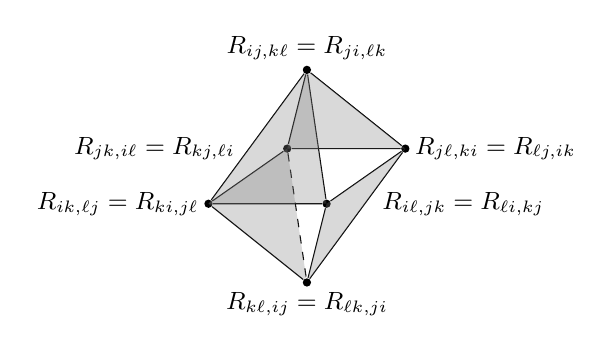
\begin{tikzpicture}
          \node [circ] (se) at (1.5, 0) {};
          \node [circ] (sw) at (0, 0) {};
          \node [circ] (ne) at (2.5, 0.7) {};
          \node [circ] (nw) at (1, 0.7) {};
          \node [circ] (top) at (1.25, 1.7) {};
          \node [circ] (bot) at (1.25, -1) {};

          \draw (sw) node [left] {\small $R_{ik, \ell j} = R_{ki, j\ell}$} -- (se) node [right] {\;\;\;\;\;\;\small $R_{i\ell, jk} = R_{\ell i, kj}$} -- (ne) node [right] {\small $R_{j\ell, ki} = R_{\ell j, ik}$} -- (nw) node [left] {\small $R_{jk, i\ell} = R_{kj, \ell i}$\;\;\;\;\;\;} -- (sw);

          \node [above] at (top) {\small $R_{ij, k\ell} = R_{ji, \ell k}$};
          \node [below] at (bot) {\small $R_{k\ell, ij} = R_{\ell k, ji}$};

          \draw (top) -- (sw) -- (bot);
          \draw (top) -- (se) -- (bot);
          \draw (top) -- (ne) -- (bot);

          \draw (top) -- (nw);
          \draw [dashed] (nw) -- (bot);

          \fill [opacity=0.3, gray] (top) -- (1.5, 0) -- (0, 0) -- (top);
          \fill [opacity=0.3, gray] (top) -- (2.5, 0.7) -- (1, 0.7) -- (top);

          \fill [opacity=0.3, gray] (bot) -- (1.5, 0) -- (2.5, 0.7) -- (bot);
          \fill [opacity=0.3, gray] (bot) -- (0, 0) -- (1, 0.7) -- (bot);
        \end{tikzpicture}
      \end{center}
      The equalities on each vertex is given by (i). By the first Bianchi idnetity, for each greyed triangle, the sum of the three vertices is zero.

      Now looking at the upper half of the octahedron, adding the two greyed triangles shows us the sum of the vertices in the horizontal square is $(-2) R_{ij, k\ell}$. Looking at the bottom half, we find that the sum of the vertices in the horizontal square is $(-2)R_{k\ell, ij}$. So we must have
      \[
        R_{ij, k\ell} = R_{k\ell, ij}.
      \]
  \end{enumerate}
\end{proof}
What exactly are the properties of the Levi-Civita connection that make these equality works? The first equality of (i) did not require anything. The second equality of (i) required the compatibility with the metric, and (ii) required the symmetric property. The last one required both properties.

We can express the last property as saying $R_{ij, k\ell}$ is a symmetric bilinear form on $\Lambda^2 T_p^*M$. It is a straightforward exercise to rewrite the statement of this proposition in coordinate free notation using test vector fields. For example, the first equality in (i) can be written as
\[
  R(X, Y) = -R(Y, X).
\]
\subsection{Sectional curvature}
Recall that if we had tangent vectors $X, Y$, then we can form
\[
  |X \wedge Y| = \sqrt{g(X, X)g(Y, Y) - g(X, Y)^2},
\]
which is the area of the parallelogram spanned by $X$ and $Y$. We now define
\[
  K(X, Y) = \frac{R(X, Y, X, Y)}{|X \wedge Y|^2}.
\]
Note that this is invariant under (non-zero) scaling of $X$ or $Y$, and is symmetric in $X$ and $Y$. Finally, it is also invariant under the transformation $(X, Y) \mapsto (X + \lambda Y, Y)$.

But it is an easy linear algebra fact that these transformations generate all isomorphism from a two-dimensional vector space to itself. So $K(X, Y)$ depends only on the $2$-plane spanned by $X, Y$. So we have in fact defined a function on the Grassmannian of $2$-planes, $K: \Gr(2, T_p M) \to \R$. This is called the \term{sectional curvature} (of $g$).

t turns out the sectional curvature determines the Riemann curvature tensor completely!
\begin{lemma}
  Let $V$ be a real vector space of dimension $\geq 2$. Suppose $R', R'': V^{\otimes 4} \to \R$ are both linear in each factor, and satisfies the symmetries we found for the Riemann curvature tensor. We define $K', K'': \Gr(2, V) \to \R$ as in the sectional curvature. If $K' = K''$, then $R' = R''$.
\end{lemma}
This is really just linear algebra.
\begin{proof}
  For any $X, Y, Z \in V$, we know
  \[
    R'(X + Z, Y, X + Z, Y) = R''(X + Z, Y, X + Z, Y).
  \]
  Using linearity of $R'$ and $R''$, and cancelling equal terms on both sides, we find
  \[
    R'(Z, Y, X, Y) + R'(X, Y, Z, Y) = R''(Z, Y, X, Y) + R''(X, Y, Z, Y).
  \]
  Now using the symmetry property of $R'$ and $R''$, this implies
  \[
    R'(X, Y, Z, Y) = R''(X, Y, Z, Y).
  \]
  Similarly, we replace $Y$ with $Y + T$, and then we get
  \[
    R'(X, Y, Z, T) + R'(X, T, Z, Y) = R''(X, Y, Z, Y) + R''"(X, T, Z, Y).
  \]
  We then rearrange and use the symmetries to get
  \[
    R'(X, Y, Z, T) - R''(X, Y, Z, T) = R'(Y, Z, X, T) - R''(Y, Z, X, T).
  \]
  We notice this equation says $R'(X, Y, Z, T) - R''(X, Y, Z, T)$ is invariant under the cyclic permutation $X \to Y \to Z \to X$. So by the first Bianchi identity, we have
  \[
    3(R'(X, Y, Z, T) - R''(X, Y, Z, T)) = 0.
  \]
  So we must have $R' = R''$.
\end{proof}

\begin{cor}
  Let $(M, g)$ be a manifold such that for all $p$, the function $K_p: \Gr(2, T_p M) \to \R$ is a constant map. Let
  \[
    R^0_p (X, Y, Z, T) = g_p(X, Z) g_p(Y, T) - g_p(X, T) g_p(Y, Z).
  \]
  Then
  \[
    R_p= K_p R_p^0.
  \]
  Here $K_p$ is just a real number, since it is constant. Moreover, $K_p$ is a smooth function of $p$.
\end{cor}

\begin{proof}
  We apply the previous lemma as follows: we define $R' = K_p R_p^0$ and $R'' = R_p$. It is a straightforward inspection to see that this $R^0$ does follow the symmetry properties of $R_p$, and that they define the same sectional curvature. So $R'' = R'$. We know $K_p$ is smooth in $p$ as both $g$ and $R$ are smooth.
\end{proof}
We can further show that if $\dim M > 2$, then $K_p$ is in fact independent of $p$ under the hypothesis of this function, and the proof requires a second Bianchi identity. This can be found on the first example sheet.

When does the condition of the corollary hold? We pick an \emph{orthonormal} basis, and express $R$ in coordinates $R_{ij, k\ell}$. Then writing $k = K_p$, the hypothesis holds iff
\[
  R_{ij, k\ell} = k(\delta_{ik}\delta_{j\ell} - \delta_{i\ell} \delta_{jk})
\]
iff
\[
  R_{ij, ij} = - R_{ij, ji} = k,
\]
and all other entries all zero.

The full curvature tensor has many components, and is rather complicated. For many purposes, it is useful to extract simpler quantities from $R_{ij, k\ell}$.
\begin{defi}[Ricci curvature]\index{Ricci curvature}\index{curvature!Ricci}
  The \emph{Ricci curvature} of $g$ at $p \in M$ is
  \[
    \Ric_p(X, Y) = \tr(v \mapsto R_p(X, v) Y).
  \]
  In terms of coordinates, we have
  \[
    \Ric_{ij} = R^q_{i,jq} = g^{pq} R_{pi, jq},
  \]
  where $g^{pq}$ denotes the inverse of $g$, and we implicitly sum over repeated indices.

  This $\Ric$ is a symmetric bilinear form on $T_p M$. This can be determined by the quadratic form
  \[
    \Ric(X) = \frac{1}{n - 1} \Ric_p(X, X).
  \]
  The coefficient $\frac{1}{n - 1}$ is just a convention.
\end{defi}
There are still two indices we can contract, and we can define
\begin{defi}[Scalar curvature]\index{scalar curvature}\index{scalar curvature}
  The \emph{scalar curvature} of $g$ is the trace of $\Ric$ respect to $g$. Explicitly, this is defined by
  \[
    s = g^{ij}\Ric_{ij} = g^{ij} R^q_{i, jq} = R^{qi}_{iq}.
  \]
\end{defi}
Sometimes a convention is to define the scalar curvature as $\frac{s}{n(n - 1})$ instead.

In the case of a constant sectional curvature tensor, we have
\[
  \Ric_p = (n - 1) K_p g_p,
\]
and
\[
  s(p) = n(n - 1) K_p.
\]

\subsection{Low dimensions}
If $n = 2$, ie. we have surfaces, then the Riemannian metric $g$ is also known as the \term{first fundamental form}, and it is usually written as
\[
  g = E\;\d u^2 + 2 F \;\d u\;\d v + G \;\d v^2.
\]
Then we find
\[
  R_{12,12} = \frac{1}{2} s (EG - F^2).
\]
Thus we find that $s/2$ is the sectional curvature. One can further check that
\[
  \frac{s}{2} = K = \frac{LN - M^2}{EG - F^2},
\]
the \term{Gaussian curvature}. We see that in two dimensions, there is only one independent component of the Gaussian curvature. We also find that $R_{12, 21}$ is the determinant of the second fundamental form.

If $n = 3$, one can check that $R(g)$ is determined by the Ricci curvature.

\section{Geodesics}
To set up the right definition of geodesics on a manifold, we need to do some preparation.

\begin{defi}[Lift]\index{lift}
  Let $\pi: E \to M$ be a vector bundle with typical fiber $V$. Consider a curve $\gamma: (-\varepsilon, \varepsilon) \to M$. A \emph{lift} of $\gamma$ is a map $\gamma^E: (-\varepsilon, \varepsilon) \to E$ if $\pi \circ \gamma^E = \gamma$:
  \[
    \begin{tikzcd}
      & E \ar[d, "\pi"]\\
      (-\varepsilon, \varepsilon) \ar[r, "\gamma"] \ar[ur, "\gamma^E"] & M
    \end{tikzcd}.
  \]
  Locally, we wlog $\gamma(t) \in U \subseteq M$ in some coordinate neighbourhood and trivializing neighbourhood of $E$. Then $\gamma^E$ is of the form
  \[
    \gamma^E(t) = (\gamma(t), a(t)),
  \]
  where $a: (-\varepsilon, \varepsilon) \to V$.
\end{defi}

\begin{defi}[Horizontal lift]\index{horizontal lift}\index{lift!horizontal}
  Let $\nabla$ be a connection on $E$ with $\Gamma^i_{jk}(x)$ the coefficients in a local trivialization. We say a lift $\gamma^E$ with local coordinates $(x(t), a(t))$ is \emph{horizontal} if
  \[
    \dot{a}^i \Gamma^i_{jk} a^j \dot{x}^k = 0.
  \] % tangent vector lies in the horizontal bundle
\end{defi}
Since this is a linear first-order ODE, by ODE theory, we know this a unique solution, and is everywhere defined as long as the coordinates are defined. Moreover, this is unique given $a(0) \in E_{\gamma(0)}$.

We can think of this operation as a function that sends $a(0)$ to $a(t)$ for some $t$. This is known as \term{parallel transport}.

\begin{defi}[Covariant derivative]\index{covariant derivative}
  Given a lift $\gamma^E(t)$ of $\gamma(t)$, we define the covariant derivative along $\gamma(t)$ as
  \[
    \left(\frac{\nabla \gamma^E}{\d t}\right)^i = \dot{a}^i + \Gamma^i_{jk} a^j \dot{x}^k.
  \]
\end{defi}

\begin{prop}
  The covariant derivative is uniquely determined, as a map between sections of $E$ along curves, by
  \begin{enumerate}
    \item
      \[
        \frac{\nabla}{\d t}(\gamma^E + c \tilde{\gamma}^E) = \frac{\nabla \gamma^E}{\d t} + c \frac{\nabla \tilde{\gamma}^E}{\d t}
      \]
      for any $c \in \R$.
    \item We have
      \[
        \frac{\nabla}{\d t}(f \gamma^E) = \frac{\d f}{\d t} + f \cdot \frac{\nabla \gamma^E}{\d t}
      \]
    \item If there is a local section $s$ of $E$ such that $\gamma^E(t) = s(\gamma(t))$ and $\dot{\gamma}(t) = V(\gamma(t))$ for $V$ a (local) vector field on $M$, then
      \[
        \frac{\nabla \gamma^E}{\d t} = (\nabla_V s) \circ \gamma.
      \]
  \end{enumerate}
\end{prop}
The proof (of a slightly less general version) can be found in III Differential Geometry.

In coordinate-free way, the condition for a lift says
\[
  \frac{\nabla \gamma^E}{\d t} = 0.
\]
Of course, we want to use this general theory to talk about the case where $M$ is a Riemannian manifold, $E = TM$ and $\nabla$ is the Levi-Civita connection of $g$. Each curve $\gamma(t)$ has a canonical lift independent of the metric or connection given simply by taking the derivative $\dot{\gamma}(t)$.
\begin{defi}[Geodesic]\index{geodesic}
  A curve $\gamma(t)$ on a Riemannian manifold $(M, g)$ is called a \emph{geodesic curve} if its canonical lift is horizontal with respect to the Levi-Civita connection. In other words, we need
  \[
    \frac{\nabla \dot{\gamma}}{\d t} = 0.
  \]
\end{defi}
In local coordinates, we write this condition as
\[
  \ddot{x}_i + \Gamma^i_{jk}\dot{x}^j \dot{x}^k = 0.
\]
This is still an ODE, but it is an equation for $x$ and not some abstract $a$. Also, this is second-order and non-linear. We still get the existence and uniqueness off solutions, but existence is only guaranteed for some interval $(-\varepsilon, \varepsilon)$. To specify a geodesic, we will have to specify $p = x(0)$ and $a = \dot{x}(0)$, and we denote the resulting geodesic as $\gamma_p(t; a)$.

We will wlog assume that
\[
  \dot{\gamma}(0) = \frac{\partial}{\partial x_1}.
\]
By the inverse function theorem, we note that $x_1(t)$ is invertible near $0$, and we can write $t = t(x_1)$ for small $x_1$. Then we can write $x_k = x_k(x_1)$, and we can now define a vector field
\[
  \dot{\underline{\gamma}}(x_1, \cdots, x_k) = \dot{\gamma}(x_1, x_2(x_1), \cdots, x_k(x_1)).
\]
Then the geodesic equation can be written as
\[
  \left.\nabla_{\dot{\underline{\gamma}}} \dot{\underline{\gamma}}\right|_{\gamma(t)} = 0.
\]
% insert picture
\begin{prop}
  If $\gamma$ is a geodesic, then $|\dot{\gamma}(t)|_g$ is constant.
\end{prop}

\begin{proof}
  We use the extension $\dot{\underline{\gamma}}$ around $p = \gamma(0)$, and stop writing the underlines. Then we have
  \[
    \dot{\gamma}(g(\dot{\gamma}, \dot{\gamma})) = g(\nabla_{\dot{\gamma}} \dot{\gamma}, \dot{\gamma})+ g(\dot{\gamma}, \nabla_{\dot{\gamma}} \dot{\gamma}) = 0,
  \]
  which is valid at each $q = \gamma(t)$ on the curve. But at each $q$, we have
  \[
    \dot{\gamma}(g(\dot{\gamma}, \dot{\gamma})) = \dot{x}^k \frac{\partial}{\partial^k} g(\dot{\gamma}, \dot{\gamma}) = \frac{\d}{\d t} |\dot{\gamma}(t)|_g^2
  \]
  by the chain rule. So we are done.
\end{proof}

For simple manifolds, geodesics are rather easy to understand.
\begin{eg}
  In $\R^n$ with the Euclidean metric, we have $\Gamma^i_{jk} = 0$. So the geodesic equation is
  \[
    \ddot{x}_k = 0.
  \]
  So the geodesics are just straight lines.
\end{eg}

\begin{eg}
  On a sphere $S^n$ with the usual metric induced by the standard embedding $S^n \hookrightarrow \R^{n + 1}$. Then we can check that the geodesics are great circles.

  To see this, we may wlog $p = e_0$ and $a = e_1$, for a standard basis $\{e_i\}$ of $\R^{n + 1}$. We can look at the map
  \[
    \varphi: (x_0, \cdots, x_n) \mapsto (x_0, x_1, -x_2, \cdots, -x_n),
  \]
  and it is clearly an isometry of the sphere. Therefore it preserves the Riemannian metric, and hence sends geodesics to geodesics. Since it also preserves $p$ and $a$, we know $\varphi(\gamma) = \gamma$ by uniqueness. So it must be contained in a great circle.
\end{eg}

We fix $p \in M$. If $\gamma(t, a)$ is a geodesic then we can observe that
\[
  \frac{\d}{\d t} \gamma(\lambda t, a) = \lambda \dot{\gamma} (\lambda t, a)
\]
by the chain rule. So we have
\[
  \frac{\d^2}{\d t^2} \gamma(\lambda t, a) = \lambda^2 \ddot{\gamma}(\lambda t, a).
\]
So we know that $\gamma(\lambda t, a) = \gamma(t, \lambda a)$, and is again a geodesic. We know solutions of ODE's depend smoothly on initial conditions. In particular, the domain $(-\varepsilon, \varepsilon)$ of $\gamma(\cdot, a)$ can be taken continuous in $a$. Thus we have $\gamma(t, a)$ is defined on $(-\varepsilon_a, \varepsilon_a)$, and $\varepsilon a > 0$ and continuous in $a \in T_p M$. When we restrict to $|a|_g \leq \varepsilon''$ for some $\varepsilon''$, we can find $\varepsilon'$ such that $\varepsilon_a \geq \varepsilon' > 0$ uniform in $a$.

Hence $\gamma(1, a) = \gamma(\varepsilon', a/\varepsilon')$ is defined for $|a|_g < \varepsilon' \varepsilon'' = \varepsilon$.

\begin{defi}[Exponential map]\index{exponential map}
  Let $(M, g)$ be a Riemannian manifold, and $p \in M$. We define $\exp_p$ by
  \[
    \exp_p(a) = \gamma(1, a) \in M
  \]
  for $a \in T_p M$ whenever this is defined.
\end{defi}
We know this function has domain at least some open ball around $0 \in T_p M$, and is smooth. Also, by construction, we have $\exp_p(0) = p$.

\begin{prop}
  We have
  \[
    (\d \exp_p)_0 = \id _{T_p M},
  \]
  where we identify $T_0 (T_p M) \cong T_p M$ in the natural way.
\end{prop}

\begin{proof}
   \[
     (\d \exp_p)_0(v) = \frac{\d}{\d t} \exp_p(tv) = \frac{\d}{\d t} \gamma(1, tv) = \frac{\d}{\d t} \gamma(t, v) = v.
   \]
\end{proof}

\begin{cor}
  $\exp_p$ maps an open ball $B(0, \delta) \subseteq T_p M$ to $U \subseteq M$ diffeomorphically for some $\delta > 0$.
\end{cor}

\begin{proof}
  By the inverse mapping theorem.
\end{proof}

This tells us the inverse of the exponenial map gives us a chart of $M$ around $p$. These coordinates are often known as \term{geodesic local coordinates}.

In these coordinates, we simply have
\[
  \gamma(t, a) = ta
\]
for all $a \in T_p M$ and $t$ sufficiently small that this makes sense.

Now consider a linear isometry $(T_p N, g(p)) \cong (\R^n, \mathrm{eucl})$, and under this identification, we have a map
\[
  (r, \mathbf{v}) \in (0, \delta) \times S^{n - 1} \mapsto \exp_p (r\mathbf{v}) \in M^n.
\]
This chart is known as \term{geodesic polar coordinates}. For each fixed $r$, the image of this map is called a \term{geodesic sphere} of geodesic radius $r$, written $\Sigma_r$\index{$\Sigma_r$}. This is an embedded submanifoldof $M$.

Note that in this chart, the metric at $0 \in T_p N$ is given by the Euclidean metric. However, the metric at other points can be complicated. Fortunately, Gauss' lemma says it is not \emph{too} complicated.

\begin{thm}[Gauss' lemma]
  The geodesic spheres are perpendicular to their radii. More precisely, $\gamma_p(t, a)$ meets every $\Sigma_r$ orthogonally, whenever this makes sense. Thus we can write the metric in geodesic polars as
  \[
    g = \d r^2 + h(r, \mathbf{v}),
  \]
  where for each $r$, we have
  \[
    h(r, \mathbf{v}) = g|_{\Sigma_r}.
  \]
  In matrix form, we have
  \[
    g =
    \begin{pmatrix}
      1 & 0 & \cdots & 0\\
      0\\
      \rvdots & & h\\
      0
    \end{pmatrix}
  \]
\end{thm}

The proof is not hard, but it involves a few subtle points.
\begin{proof}
  We work in geodesic coordinates. It is clear that $g(\partial_r, \partial_r) = 1$.
  
  Consider an arbitrary vector field $X = X(\mathbf{v})$ on $S^{n - 1}$. This induces a vector field on some neighbourhood $B(0, \delta) \subseteq T_p M$ by
  \[
    \tilde{X}(r\mathbf{v}) = X(\mathbf{v}).
  \]
  Pick a direction $\mathbf{v} \in T_pM$, and consider the unit speed geodesic $\gamma$ in the direction of $\mathbf{v}$. We define
  \[
    G(r) = g(\tilde{X}(r\mathbf{v}), \dot{\gamma}(r)) = g(\tilde{X}, \dot{\gamma}(r)).
  \]
  We begin by noticing that
  \[
    \nabla_{\partial_r} \tilde{X} - \nabla_{\tilde{X}} \partial_r = [\partial_r , \tilde{X}] = 0.
  \]
  So we have
  \[
    \frac{\d}{\d r} G(r) = g(\nabla_{\dot{\gamma}} \tilde{X}, \dot{\gamma}) + g(\tilde{X}, \nabla_{\dot{\gamma}} \dot{\gamma}).
  \]
  We know the second term vanishes, since $\gamma$ is a geodesic. Noting that $\dot{\gamma} = \frac{\partial}{\partial r}$, we know the first term is equal to
  \[
    g(\nabla_{\tilde{X}} \partial_r, \partial_r) = \frac{1}{2} \big(g(\nabla_{\tilde{X}} \partial_r, \partial_r) + g( \partial_r, \nabla_{\tilde{X}}\partial_r)\big) = \frac{1}{2} \tilde{X} (g(\partial_r, \partial_r)) = 0,
  \]
  since we know that $g(\partial_r, \partial_r) = 1$ constantly.

  Thus, we know $G(r)$ is constant. But $G(0) = 0$ since the metric at $0$ is the Euclidean metric. So $G$ vanishes everywhere, and so $\partial_r$ is perpendicular to 

%
%  We work in the geodesic coordinates. Consider an arbitrary vector field $X = X(\mathbf{v}) \in \Vect(S^{n - 1})$. Identifying $S^{n - 1} \subseteq T_p M$, we extend this to a vector field on $B(0,\delta) \subseteq T_p M$ by
%  \[
%    \tilde{X}(r\mathbf{v}) = r X(\mathbf{v}).
%  \]
%  We want to show that $\tilde{X}$ is perpendicular $\frac{\partial}{\partial r}$ at each point in $B \setminus \{0\}$. Consider an arbitrary unit speed geodesic $\gamma$ in direction $\mathbf{v}$. We define the quantity
%  \[
%    G(r) = g(\tilde{X}(r\mathbf{v}), \dot{\gamma}(r)).
%  \]
%  We will show that $G$ vanishes everywhere. To do so, we claim that
%  \[
%    \frac{\d G}{\d r} = \frac{G}{r}.
%  \]
%  It then follows that $G$ is linear in $r$, 
%
%
%  This is equivalent to showing that it is perpendicular to $\dot{\gamma}$. Recall that we have
%  \[
%    \nabla_{\dot{\gamma}} \dot{\gamma} = 0
%  \]
%  by definition. Also, we know $\frac{\partial}{\partial r}$ has unit norm. Thus to show that
%  \[
%    g(\tilde{X}, \dot{\gamma}) = 0
%  \]
%
%  We consider
%  \[
%    \nabla_{\partial/\partial r} \tilde{X} - \nabla_{\tilde{X}} \frac{\partial}{\partial r} = \left[\frac{\partial}{\partial r}, \tilde{X}\right] =  \frac{\d}{\d r}\tilde{X} = \frac{\tilde{X}}{r}.
%  \]
%  We also have
%  \begin{align*}
%    \frac{\d}{\d r} (g(\tilde{X}, \dot{\gamma})) &= g(\nabla_{\dot{\gamma}} \tilde{X}, \dot{\gamma})  + g(\tilde{X}, \nabla_{\dot{\gamma}} \dot{\gamma})\\
%    &= -g\left(\nabla_{\tilde{X}} \dot{\gamma} + \frac{\tilde{X}}{r}, \dot{\gamma}\right) = \frac{1}{r} g(Y, \dot{~g}),
%  \end{align*}
%  noting that $g(\nabla_{\tilde{X}} \dot{\gamma}, \dot{\gamma}) = Y g(\dot{\gamma}, \dot{\gamma}) = 0$ since $|\dot{\gamma}|$ is constant along spheres. We define
%  \[
%    G = g(\tilde{X}, \dot{\gamma}).
%  \]
%  Then we know this satisfies
%  \[
%    \frac{\d}{\d r} G = \frac{G}{r}.
%  \]
%  This is a very simple ODE in $r$, and this tells us $G$ is linear in $r$. So
%  \[
%    \frac{\d G}{\d r}
%  \]
%  is independent of $r$. But as $r \to 0$, we know
%  \[
%    \lim_{r \to 0} \frac{\d G}{\d r} = \lim_{r \to 0} g\left(X, \frac{\partial}{\partial r}\right) = 0.
%  \]
\end{proof}

\begin{cor}
  Let $a, w \in T_p M$. Then
  \[
    g((\d \exp_p)_a a, (\d \exp_p)_a w) = g(a, w)
  \]
  whenever this makes sense.
\end{cor}

\section{Jacobi fields}
Jacobi fields are special vector fields along geodesic curves. To talk about them, it is convenient to talk about one-parameter families of geodesic curves.

Pick $a \in T_p M$, and define
\[
  a(s): (-\varepsilon, \varepsilon) \to T_p N
\]
such that $a(0) = a$ and $\dot{a}(0) = w \in T_a(T_p M) \cong T_p M$. We may extend $r$ and $s$ to a set of local coordinates. Consider the following function:
\[
  f(t, s) = \exp_p(t a(s)).
\]
Then we have
\[
  (\d \exp_p)_a w = \left.\frac{\partial f}{\partial s}\right|_{(1, 0)}.
\]
We shall be interested in
\[
  \frac{\partial f}{\partial s}.
\]
More generally, we have
\[
  (\d \exp_p)_{t a_0} (tw) = \frac{\partial f}{\partial s}(t, 0),
\]
which is a vector field along $\gamma = \gamma_p(t, a) = \exp(ta)$. This is the restriction of $\frac{\partial}{\partial s}$ to $\gamma_p(\cdot, a)$.

Recall that the geodesic equations say
\[
  \frac{\nabla}{\d t} \dot{\gamma} = 0.
\]
Also, notice that in the present set up, we have 
\[
  \dot{\gamma} = \frac{\partial f}{\partial t} = \frac{\partial}{\partial t},
\]
and this is defined on an open domain. Therefore, we can write
\begin{align*}
  0 = \nabla_{\partial_s} \nabla_{\partial_t} \frac{\partial}{\partial t} &= \nabla_{\partial t} \nabla_{\partial_s} \partial_t - R(\partial_s, \partial_t) \partial_t\\
  &=  \nabla_{\partial t} \nabla_{\partial_s} \partial_t + R(\partial_t, \partial_s) \partial_t\\
\end{align*}
We let this act on the function $f$. So we get
\[
  \frac{\nabla}{\d t} \frac{\nabla}{\d s} \frac{\partial f}{\partial t} + R(\partial_t, \partial_s) \frac{\partial f}{\partial t}.
\]
We write
\[
  J(t) = \frac{\partial f}{\partial s}(t, 0),
\]
which is a vector field along the geodesic $\gamma$. We then find that $J$ must satisfy the ordinary differential equation
\[
  \frac{\nabla^2}{\d t^2} J + R(\dot{\gamma}, J) \dot{\gamma} = 0 \tag{$\dagger$}.
\]
Here we used the fact that
\[
  \frac{\nabla}{\d s} \frac{\partial f}{\partial t} = \frac{\nabla}{\d t} \frac{\partial f}{\partial s}.
\]
This is a linear second-order ordinary differential equation.

\begin{defi}[Jacobi field]\index{Jacobi field}
  Let $\gamma: [0, L] \to M$ be a geodesic. A \emph{Jacobi field} is a vector field $J$ along $\gamma$ that is a solution of the Jacobi equation on $[0, L]$
  \[
    \frac{\nabla^2}{\d t^2} J + R(\dot{\gamma}, J) \dot{\gamma} = 0 \tag{$\dagger$}.
  \]
\end{defi}

Observe that $\dot{\gamma}(t)$ and $t \dot{\gamma}(t)$ both satisfy this equation, rather trivially.
\begin{thm}
  Let $\gamma: [0, L] \to N$ be a geodesic in a Riemannian manifold $(M, g)$. Then
  \begin{enumerate}
    \item For any $u, v \in T_{\gamma(0)}M$, there is a unique Jacobi field $J$ along $\Gamma$ with
      \[
        J(0) = u,\quad \frac{\nabla J}{\d t}(0) = v.
      \]
      If
      \[
        J(0) = 0, \frac{\nabla J}{\d t}(0) = k \dot{\gamma}(0),
      \]
      then $J(t) = kt \dot{\gamma}(t)$. Moreover, if both $J(0), \frac{\nabla J}{\d t}(0)$ are orthogonal to $\dot{\gamma}(0)$, then $J(t)$ is perpendicular to $\dot{\gamma}(t)$ for all $[0, L]$.

      In particular, the vector space of all Jacobi fields along $\gamma$ have dimension $2n$, where $n = \dim M$.

      The subspace of those Jacobi fields pointwise perpendicular to $\dot{\gamma}(t)$ has dimensional $2(n - 1)$.
    \item $J(t)$ is independent of the parametrization of $\dot{\gamma}(t)$. Explicitly, if $\tilde{\gamma}(t) = \tilde{\gamma}(\lambda t)$, then $\tilde{J}$ with the same initial conditions as $J$ is given by
      \[
        \tilde{J}(\tilde{\gamma}(t)) = J(\gamma(\lambda t)).
      \]
  \end{enumerate}
\end{thm}

\begin{proof}\leavevmode
  \begin{enumerate}
    \item Pick an orthonormal $e_1,\cdots, e_n$ of $T_p M$, where $p = \gamma(0)$. Then parallel transports $\{X_i(t)\}$ via the Levi-Civita connection preserves the inner product.

      We take $e_1$ to be parallel to $\dot{\gamma}(0)$. By definition, we have
      \[
        X_i(0) = e_i,\quad \frac{\nabla X_i}{\d t} = 0.
      \]
      Now we can write
      \[
        J = \sum_{i = 1}^n y_i X_i.
      \]
      Then taking $g(X_i, \cdot)$ of $(\dagger)$ , we find that
      \[
        \ddot{y}_i + \sum_{j = 2}^n R(\dot{\gamma}, X_j, \dot{\gamma}, X_i) y_j = 0.
      \]
      Then the claims of the theorem follow from the standard existence and uniqueness of solutions of differential equations.
      
      In particular, for the orthogonality part, we know that $J(0)$ and $\frac{\nabla J}{\d t}(0)$ being perpendicular to $\dot{\gamma}$ is equivalent to $y_1(0) = \dot{y}_1 (0) = 0$, and then Jacobi's equation gives
      \[
        \ddot{y}_1(t) = 0.
      \]
    \item This follows from uniqueness.
  \end{enumerate}
\end{proof}

In the case where we have a constant sectional curvature, it is easy to determine all Jacobi fields explicitly.

\begin{eg}
  Suppose the sectional curvature is constantly $K \in \R$, for $\dim M \geq 3$. We wlog $|\dot{\gamma}| = 1$. We let $J$ along $\gamma$ be a Jacobi field, normal to $\dot{\gamma}$.
  
  Then for any vector field $T$ along $\gamma$, we have
  \[
    \bra R(\dot{\gamma}, J) \dot{\gamma}, T\ket = K(g(\dot{\gamma}, \dot{\gamma}) g(J, T) - g(\dot{\gamma}, J) g(\dot{\gamma}, T)) = K g(J, T).
  \]
  Since this is true for all $T$, we know
  \[
    R(\dot{\gamma}, J) \dot{\gamma} = KJ.
  \]
  Then the Jacobi equation becomes
  \[
    \frac{\nabla^2}{\d t^2}J + KJ = 0.
  \]
  So we can immediately write down a collection of solutions
  \[
    J(t) =
    \begin{cases}
      \frac{\sin(t \sqrt{K})}{\sqrt{K}} X_i(t)  & K > 0\\
      t X_i(t) & K = 0\\
      \frac{\sinh(t \sqrt{-K})}{\sqrt{-K}} X_i(t) & K < 0
    \end{cases}.
  \]
  for $i = 2, \cdots, n$, and this has initial conditions
  \[
    J(0) = 0,\quad \frac{\nabla J}{\d t}(0) = e_i.
  \]
  This gives a Jacobi field that vanishes at $0$.
\end{eg}

\begin{prop}
  Let $\gamma: [a, b] \to M$ be a geodesic, and $f(t, s)$ a variation of $\gamma(t) = f(t, 0)$ such that $f(t, s) = \gamma_s(t)$ is a geodesic for all $|s|$ small. Then
  \[
    J(t) = \frac{\partial f}{\partial s}
  \]
  is a Jacobi field along $\dot{\gamma}$.

  Conversely, every Jacobi field along $\gamma$ can be obtained this way for an appropriate function $f$.
\end{prop}
So Jacobi fields are precisely the variations of geodesics.

\begin{proof}
  As before, we have
  \begin{align*}
    \frac{\nabla^2 J}{\d t} &= \nabla_t \nabla_t \frac{\partial f}{\partial s}\\
    &= \nabla_t \nabla_s \frac{\partial f}{\partial t}\\
    &= \nabla_s \left(\nabla_t \frac{\partial f}{\partial t}\right) - R(\partial_t, \partial_s) \dot{\gamma}_s.
  \end{align*}
  We notice that the first term vanishes, because $\nabla_t \frac{\partial f}{\partial t} = 0$ by definition of geodesic. So we find
  \[
    \frac{\nabla^2 J}{\d t} = -R(\dot{\gamma}, J) \dot{\gamma},
  \]
  which is the Jacobi equation.

  The converse requires a bit more work. We will write $J'(0)$ for the convavriant derivative of $J$ along $\gamma$.

  Given a Jacobi field $J$ along a geodesic $\gamma(t)$ for $t \in [0, L]$, we let $\tilde{\gamma}$ be another geodesic such that
  \[
    \tilde{\gamma}(0) = \gamma(0),\quad \dot{\tilde{\gamma}}(0)  = J(0).
  \]
  We take parallel vector fields $X_0, X_1$ along $\tilde{\gamma}$ such that
  \[
    X_0(0) = \dot{\gamma}(0), X_1(0) = J'(0).
  \]
  We put $X(s) = X_0(s) + s X_1(s)$. We put
  \[
    f(t, s) = \exp_{\tilde{\gamma}(s)} (t X(s)).
  \]
  In local coordiantes, we find
  \[
    f(t, s) = \dot{\gamma}(s) + t X(s) + O(t^2)
  \]
  as $t \to 0$, with $s$ fixed. Then we define
  \[
    \gamma_s(t) = f(t, s)
  \]
  whenever this makes sense, and this depends smoothly on $s$. The previous arguments say we get a Jacobi field
  \[
    \hat{J}(t) = \frac{\partial f}{\partial s}(t, 0)
  \]
  We now want to check that $\hat{J} = J$. Then we are done. To do so, we have to check the initial conditions. We have
  \[
    \hat{J}(0) = \frac{\partial f}{\partial s}(0, 0) = \frac{\d \tilde{\gamma}}{\d s}(0) = J(0),
  \]
  and also 
  \[
    \hat{J}'(0) = \frac{\nabla}{\d t} = \frac{\partial f}{\partial s}(0, 0) = \frac{\nabla}{\d s} \frac{\partial f}{\partial t}(0, 0) = \frac{\nabla X}{\d s}(0) = X_1(0) = J'(0).
  \]
  So we have $\hat{J} = J$.
\end{proof}

\begin{cor}
  Every Jacobi field $J$ along a geodesic $\gamma$ with $J(0) = 0$ is given by
  \[
    J(t) = (\d \exp_p)_{t \dot{\gamma}(0)} (t J'(0))
  \]
  for all $t \in [0, L]$.
\end{cor}

\begin{proof}
  Write $\dot{\gamma}(0) = a$, and $J'(0) = w$. By above, we can construct the variation by
  \[
    f(t, s) = \exp_p(t (a + sw)).
  \]
  Then
  \[
    (\d \exp_p)_{t(a + sw)} (tw) = \frac{\partial f}{\partial s}(t, s),
  \]
  which is just an application of the chain rule. Putting $s = 0$ gives the result.
\end{proof}

It can be shown that in the situation of the corollary, if $a \perp w$, and $|a| = |w| = 1$, then
\[
  |J(t)| = t - \frac{1}{3!} K(\sigma) T^3 + o(t^3)
\]
as $t \to 0$, where $\sigma$ is the plane spanned by $a$ and $w$.

We now revisit the Gauss lemma, and deduce a stronger version.
\begin{lemma}[Gauss' lemma]\index{Gauss' lemma}
  Let $a, w \in T_p M$, and
  \[
    \gamma = \gamma_p(t, a) = \exp_p(ta)
  \]
  a geodesic. Then
  \[
    g_{\gamma(t)} ((\d \exp_p)_{ta} a, (\d \exp_p)_{ta} w) = g_{\gamma(0)}(a, w).
  \]
  In particular, $\gamma$ is orthogonal to $\exp_p \{v \in T_p M: |v| = r\}$. Note that the latter need not be a submanifold.
\end{lemma}
This is an improvement of the previous version, which required us to live in the geodesic polar coordinates.

\begin{proof}
  Consider the Jacobi field $J$ satisfying
  \[
    J(0) = 0,\quad J'(0) = \frac{w}{r}.
  \]
  Then by the corollary, we knkow the Jacobi field is
  \[
    J(t) = (\d \exp_p)_{ta} \left(\frac{tw}{r}\right).
  \]
  We may write
  \[
    \frac{w}{r} = \lambda a + u,
  \]
  with $a \perp u$. Then since Jacobi fields depend linearly on initial conditions, we  write
  \[
    J(t) = a\lambda t \dot{\gamma}(t) + J_n(t)
  \]
  for a Jacobi field $J_n$ a normal vector field along $\gamma$. So we have
  \[
    \gamma(J(r), \dot{\gamma}(r)) = \lambda r |\dot{\gamma}(r)|^2 = g(w, a).
  \]
  Now we use the fact that
  \[
    J(r) = (\d \exp_p)_{ra} w
  \]
  and
  \[
    \dot{\gamma}(r) = (\d \exp_p)_{ra} a,
  \]
  and we are done.
\end{proof}

\begin{cor}[Local minimizing of length]
  Let $a \in T_p M$. We define $\varphi(t) = ta$, and $\psi(t)$ a $C^1$ curve in $T_p M$ for $t \in [0, 1]$ such that
  \[
    \psi(0) = 0,\quad \psi(1) = a.
  \]
  Then
  \[
    \length(\exp_p \circ \psi) \geq \length(\exp \circ \varphi) = |a|.
  \]
\end{cor}
So we see that geodesics minimize length, as long as we live inside the image of the exponential map.
\begin{proof}
  We write
  \[
    \psi(t) = \rho(t) \mathbf{u}(t), 
  \]
  where $\rho(t) \geq 0$ and $|\mathbf{u}(t)| = 1$. Then
  \[
    \psi' = \rho' \mathbf{u} + \rho \mathbf{u}'.
  \]
  So we have
  \[
    \left|\frac{\d}{\d x} (\exp_p \circ \psi) (t)\right|^2 = \left|(\d \exp_p)_{\psi(t)} \psi'(t) \right|^2 = \rho'(t)^2 + \rho(t)^2 |(\d \exp_p)_{\psi(t)} \mathbf{u}'(t)|^2,
  \]
  using the extended Gauss lemma. Then we find that
  \[
    \length(\exp_p \circ \psi) \geq \int_0^1 \rho'(t) \;\d t = \rho(1) - \rho(0) = |a|.
  \]
\end{proof}

\begin{defi}[Distance]\index{distance}
  Suppose $M$ is connected, which is the same as it being path connected. Let $(p, q) \in M$. We define
  \[
    d(p, q) = \inf_{\xi \in \Omega(p, q)} \length(\xi),
  \]
  where $\Omega(p, q)$ is the set of all piecewise $C^1$ curves from $p$ to $q$.
\end{defi}

We note that $\Omega(p, q)$ has a topology, given by the topology of uniform convergence, given by this distance $d$.

\begin{thm}
  Let $\gamma(t) = \exp_p(ta)$ be a geodesic, for $t \in [0, 1]$. Let $q = \gamma(1)$. Assume $ta$ is a regular point for $\exp_p$ for all $t \in [0, 1]$. Then there exists a neighbourhood of $\gamma$ in $\Omega(p, q)$ such that for all $\psi$ in this neighbourhood, $\ell(\psi) \geq \ell(\gamma)$, with equality iff $\psi = \gamma$ up to reparametrization.
\end{thm}
Note that the condition that $ta$ is regular is crucial, eg. we can take a sphere, and consider $p, q$ to be antipodal points. Note also that $\gamma$ is only the local minimizer.

\end{document}
